 \documentclass[a4paper, 11pt]{article}
\usepackage{comment} 
\usepackage{fullpage}
\usepackage{times}
\usepackage{amsmath,amssymb,amsfonts,textcomp}
\usepackage{graphicx}
\usepackage{float,flafter}
\usepackage{hyperref}
\usepackage{inputenc}
\usepackage[]{algorithm2e}
\usepackage{xcolor}
\usepackage[flushleft]{threeparttable}
\usepackage{graphicx}
\usepackage{float}
\usepackage{subcaption}
\graphicspath{ {./images/} }
\begin{document}
\begin{center}
\hrule

\vspace{.4cm}
{\bf {\Huge Data Mining Project}}\\
\vspace{.2cm}
{Mohammed Zaki Nassar}  
\end{center}
\hrule

\section{Problem understanding}
	
	In our dataset we have a lot of details about students' lives, who study math and Portuguese language in a secondary school. The data was collected via a survey of the students in question.
	I am going to take a deeper look at the composition of the students in the data set. And then take a look at how different aspects of their lives affect their final grades. And, of course, take a look at how alcohol consumption can affect the success of students as well.
	
	The data contains 1044 entries, with 33 observations. This amount of details can provide a chance to take a closer look at what affects the success of students in their education and what other factors are of no consequence when it comes to final grades in secondary school tests.

\section{Data understanding}
	As a first step we take a look at the composition of the students by gender and age:
	
	\begin{figure}[h!]
		\centering
		\begin{subfigure}[b]{0.4\linewidth}
			\hspace*{-1.0in}
			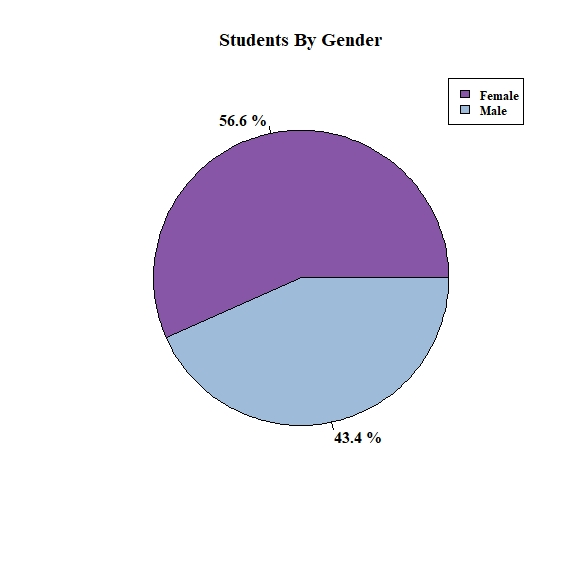
\includegraphics[width=1.5\linewidth]{gender.jpeg}
		\end{subfigure}
		\begin{subfigure}[b]{0.4\linewidth}
			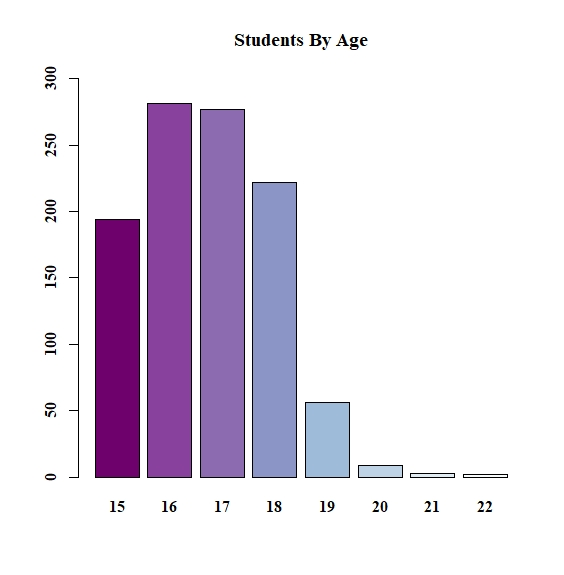
\includegraphics[width=1.5\linewidth]{age.jpeg}
		\end{subfigure}
		\caption*{Students by gendre and age.}
		\label{fig:gender_age}
	\end{figure}
	

	So, we are dealing a an age range of mostly teenagers between 15-18 years old, where the number of girls a little more, but not by a huge margin.
	
\section{Data Preparation}
	
	For the data preparation we try to find the factors that affect the students grades the most. So, we start with a correlation graph: 
	\begin{center}
		\begin{figure}[H]
			\hspace*{1.5in}
			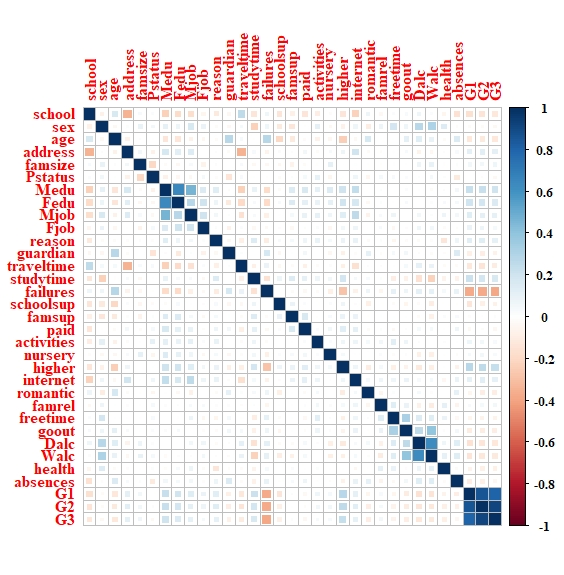
\includegraphics[width=222px]{correlation.jpeg}
			\label{fig:correlation}
		\end{figure}
	\end{center}
	
	Now, we can take a closer look at some of the variables that affect the grades the most and some others that I suspect can be of some significance. 
	First, let's take a look at how long does it take most students to get to school and back home:
	\begin{center}
		\begin{figure}[H]
			\hspace*{1.5in}
			\vspace*{-0.5in}
			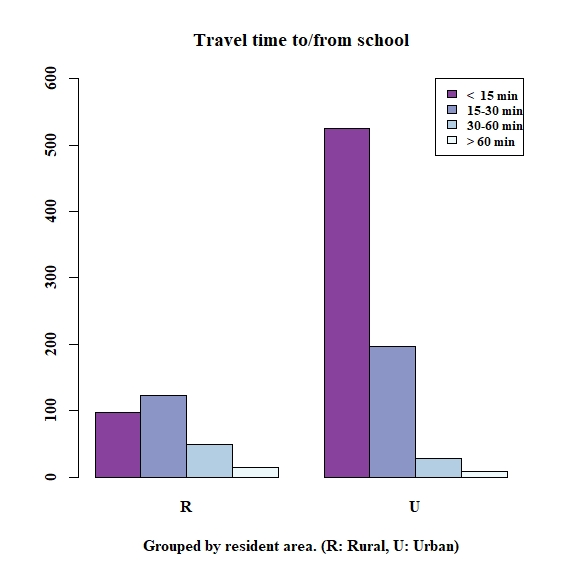
\includegraphics[width=222px]{travel_time.jpeg}
			\label{fig:travel_time}
		\end{figure}
	\end{center}
	
	Let's take a look at how this travel time affects the number of absences from school:
	\begin{figure}[H]
		\centering
		\begin{subfigure}[b]{0.4\linewidth}
			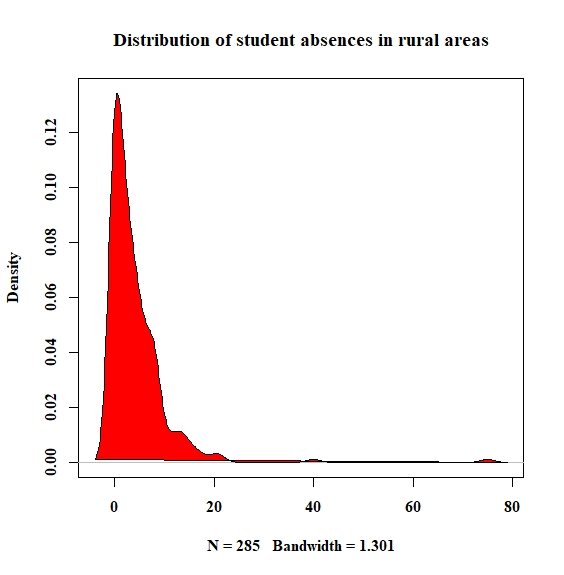
\includegraphics[width=\linewidth]{abs_rur.jpeg}
		\end{subfigure}
		\begin{subfigure}[b]{0.4\linewidth}
			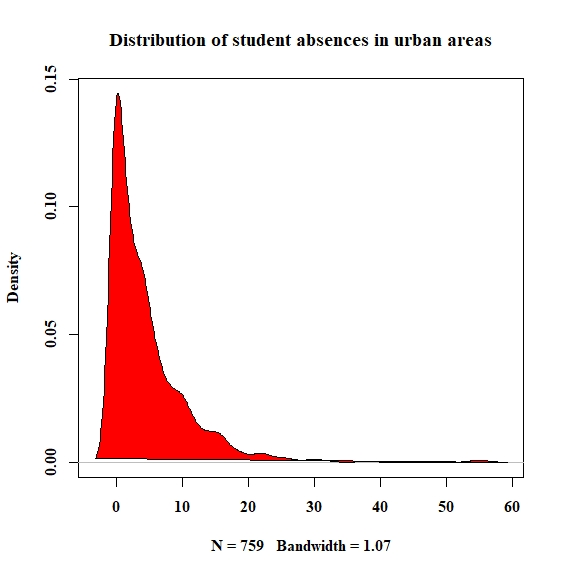
\includegraphics[width=\linewidth]{abs_urb.jpeg}
		\end{subfigure}
		\caption*{Distribution of absences for students by urban and rural residence.}
		\label{fig:absences}
	\end{figure}
	
	We can notice that students in rural areas have a slightly higher percentage of absences compared to city students. However, this can be attributed to factors other than their distance from school.
	\\
	
	One of the most important factors, of course, is the amount of time the student spends each week on his studies. In the following graph we see the students by their reported time spent studying each week and a box plot showing the correlation between this time and the final grade:
	
	\begin{figure}[h!]
		\centering
		\begin{subfigure}[b]{0.4\linewidth}
			\hspace*{-1.2in}
			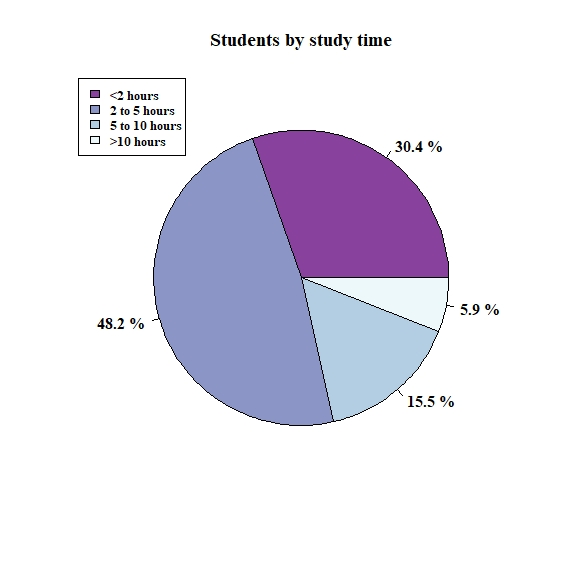
\includegraphics[width=1.5\linewidth]{study_time.jpeg}
		\end{subfigure}
		\begin{subfigure}[b]{0.4\linewidth}
			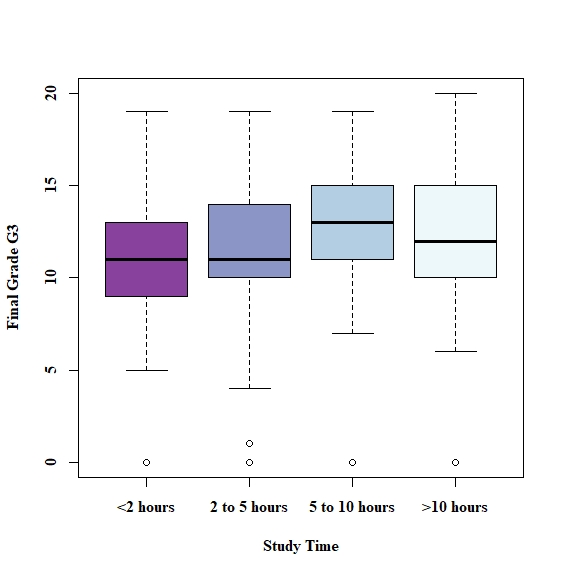
\includegraphics[width=1.5\linewidth]{study_time_grades.jpeg}
		\end{subfigure}
		\caption*{Study time and final grades.}
		\label{fig:study_time_grades}
	\end{figure}
	
	As expected, less than two hours per week for studying is not enough time to get high grades, and higher grades are correlated with more studying. We can also notice that the number of students spending more than 10 hours per week studying is low. But they achieve the highest average of grades.
	\\
	Another factor to look into is the students' health:
	
	\begin{figure}[h!]
		\centering
		\begin{subfigure}[b]{0.4\linewidth}
			\hspace*{-1.2in}
			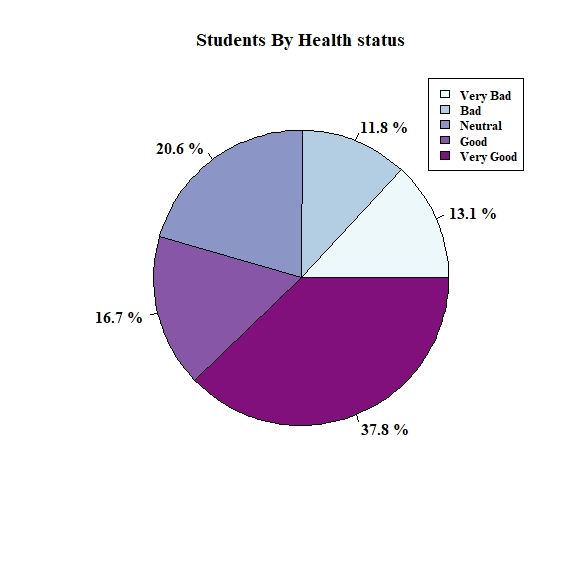
\includegraphics[width=1.5\linewidth]{health.jpeg}
		\end{subfigure}
		\begin{subfigure}[b]{0.4\linewidth}
			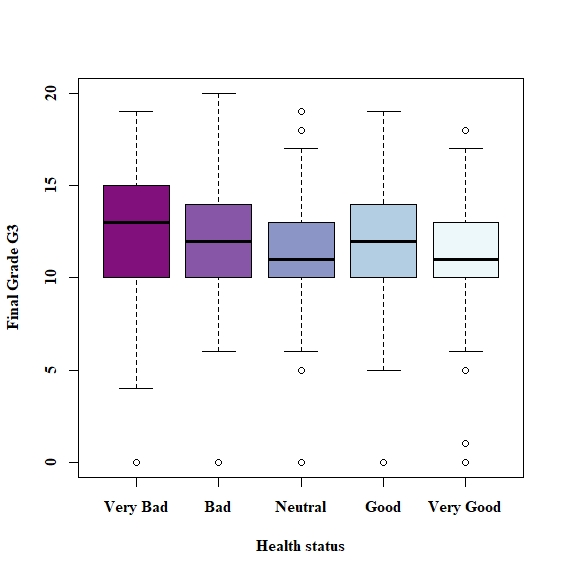
\includegraphics[width=1.5\linewidth]{health_grades.jpeg}
		\end{subfigure}
		\caption*{Health status and final grades.}
		\label{fig:health_grades}
	\end{figure}

	An interesting observation is that students who report bad health status have high average grades. Which could suggest that their efforts to excel at school is at the expense of their health.
	\\
	
	Now we analyse how alcohol consumption affects students' performance. First, we look at their weekday consumption: 
	
	\begin{figure}[H]
		\centering
		\begin{subfigure}[b]{0.3\linewidth}
			\hspace*{-1.2in}
			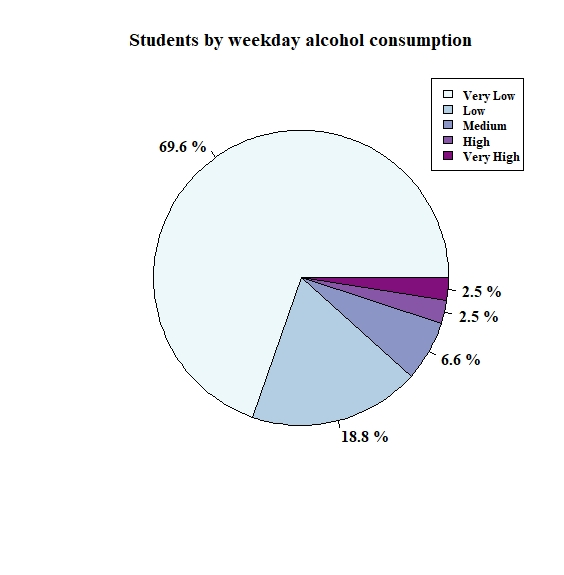
\includegraphics[width=1.6\linewidth]{weekday_alcohol.jpeg}
		\end{subfigure}
		\begin{subfigure}[b]{0.3\linewidth}
			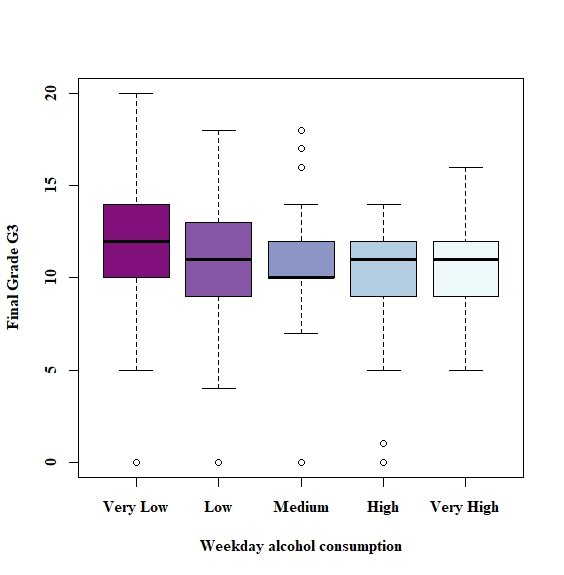
\includegraphics[width=1.6\linewidth]{weekday_alcohol_grades.jpeg}
		\end{subfigure}
		\caption*{Weekday alcohol consumption and final grades.}
		\label{fig:weekday_alcohol_grades}
	\end{figure}

	So clearly, we can see how weekday alcohol consumption negatively affects the students grades. And thankfully, most students prefer little to no alcohol during the week.
	\\
	
	We also take a look at the weekend alcohol consumption and its effects:
	
	\begin{figure}[h!]
		\centering
		\begin{subfigure}[b]{0.4\linewidth}
			\hspace*{-1.2in}
			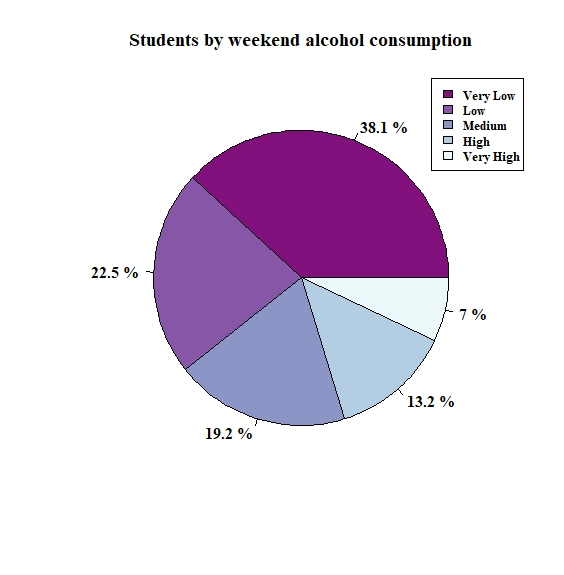
\includegraphics[width=1.5\linewidth]{weekend_alcohol.jpeg}
		\end{subfigure}
		\begin{subfigure}[b]{0.4\linewidth}
			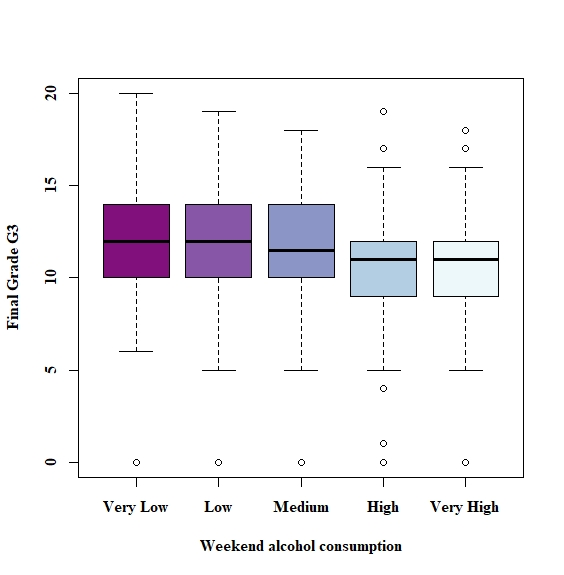
\includegraphics[width=1.5\linewidth]{weekend_alcohol_grades.jpeg}
		\end{subfigure}
		\caption*{Weekend alcohol consumption and final grades.}
		\label{fig:weekend_alcohol_grades}
	\end{figure}
	
	For the weekend, alcohol consumption increases among students. However, it doesn't show that it affects the students' grades as long as they don't abuse it.
	\\
	
	One final factor to consider is the student's desire for a higher education and how would that desire motivate his performance:
	
	\begin{figure}[h!]
		\centering
		\begin{subfigure}[b]{0.2\linewidth}
			\hspace*{-1.6in}
			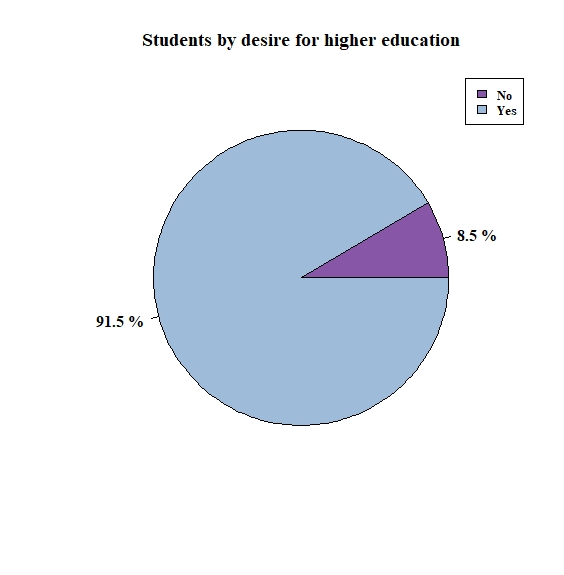
\includegraphics[width=2.0\linewidth]{higher.jpeg}
		\end{subfigure}
		\begin{subfigure}[b]{0.2\linewidth}
			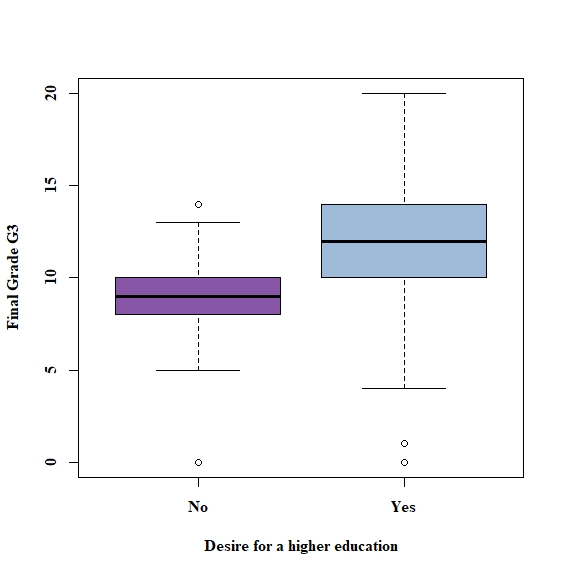
\includegraphics[width=2.0\linewidth]{higher_grades.jpeg}
		\end{subfigure}
		\caption*{Higher education desire and final grades.}
		\label{fig:higher_grades}
	\end{figure}
	
	As it's quite apparent, the desire for a higher education motivates the students to increase their performance in secondary school.
	
	
	\section{Modeling}
	
	For modeling, a linear regression model was created based on the most significant factors found from the analysis above. And these factors are: 
	\begin{itemize}
		\item Study time
		\item Health status
		\item Weekday alcohol consumption.
	\end{itemize}

	With the following model:
	
	\begin{center}
		\begin{figure}[H]
			\hspace*{1.2in}
			\vspace*{-0.5in}
			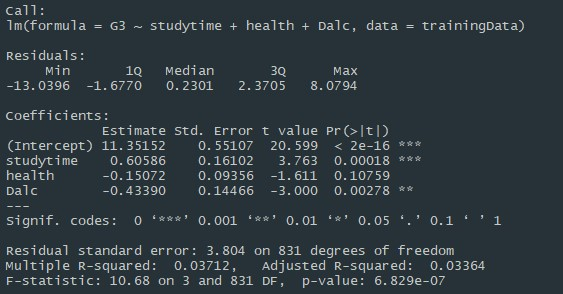
\includegraphics[width=300px]{model.jpeg}
			\label{fig:model}
		\end{figure}
	\end{center}

	\section{Evaluation}
	
	For the evaluation of the model, the test subset was use for prediction with the following results:
	
	\begin{table}[H]
		\centering
		\begin{tabular}{|l|l|l|}
			\hline
			& Actual Values & Predicts \\ \hline
			7  & 13            & 11.67718 \\ \hline
			8  & 13            & 11.97862 \\ \hline
			10 & 13            & 11.37574 \\ \hline
			14 & 13            & 11.67718 \\ \hline
			20 & 12            & 10.76988 \\ \hline
		\end{tabular}
	\end{table}
	
	
	
\end{document}